\section{Vorlesung 25.11.2016}
\subsection{Färbung von Graphen}
\textbf{Vertexfärbung}\newline
Zwei durch eine Kante verbundene Knoten haben unterschiedliche Farben. \newline
Beispiel wäre eine Landkarte auf der mit so wenig wie möglich Farben die Länder ausgemalt werden, ohne zwei benachbarte Länder gleichfarbig zu haben. Hierbei entspricht jede Facette einen Knoten.\newline
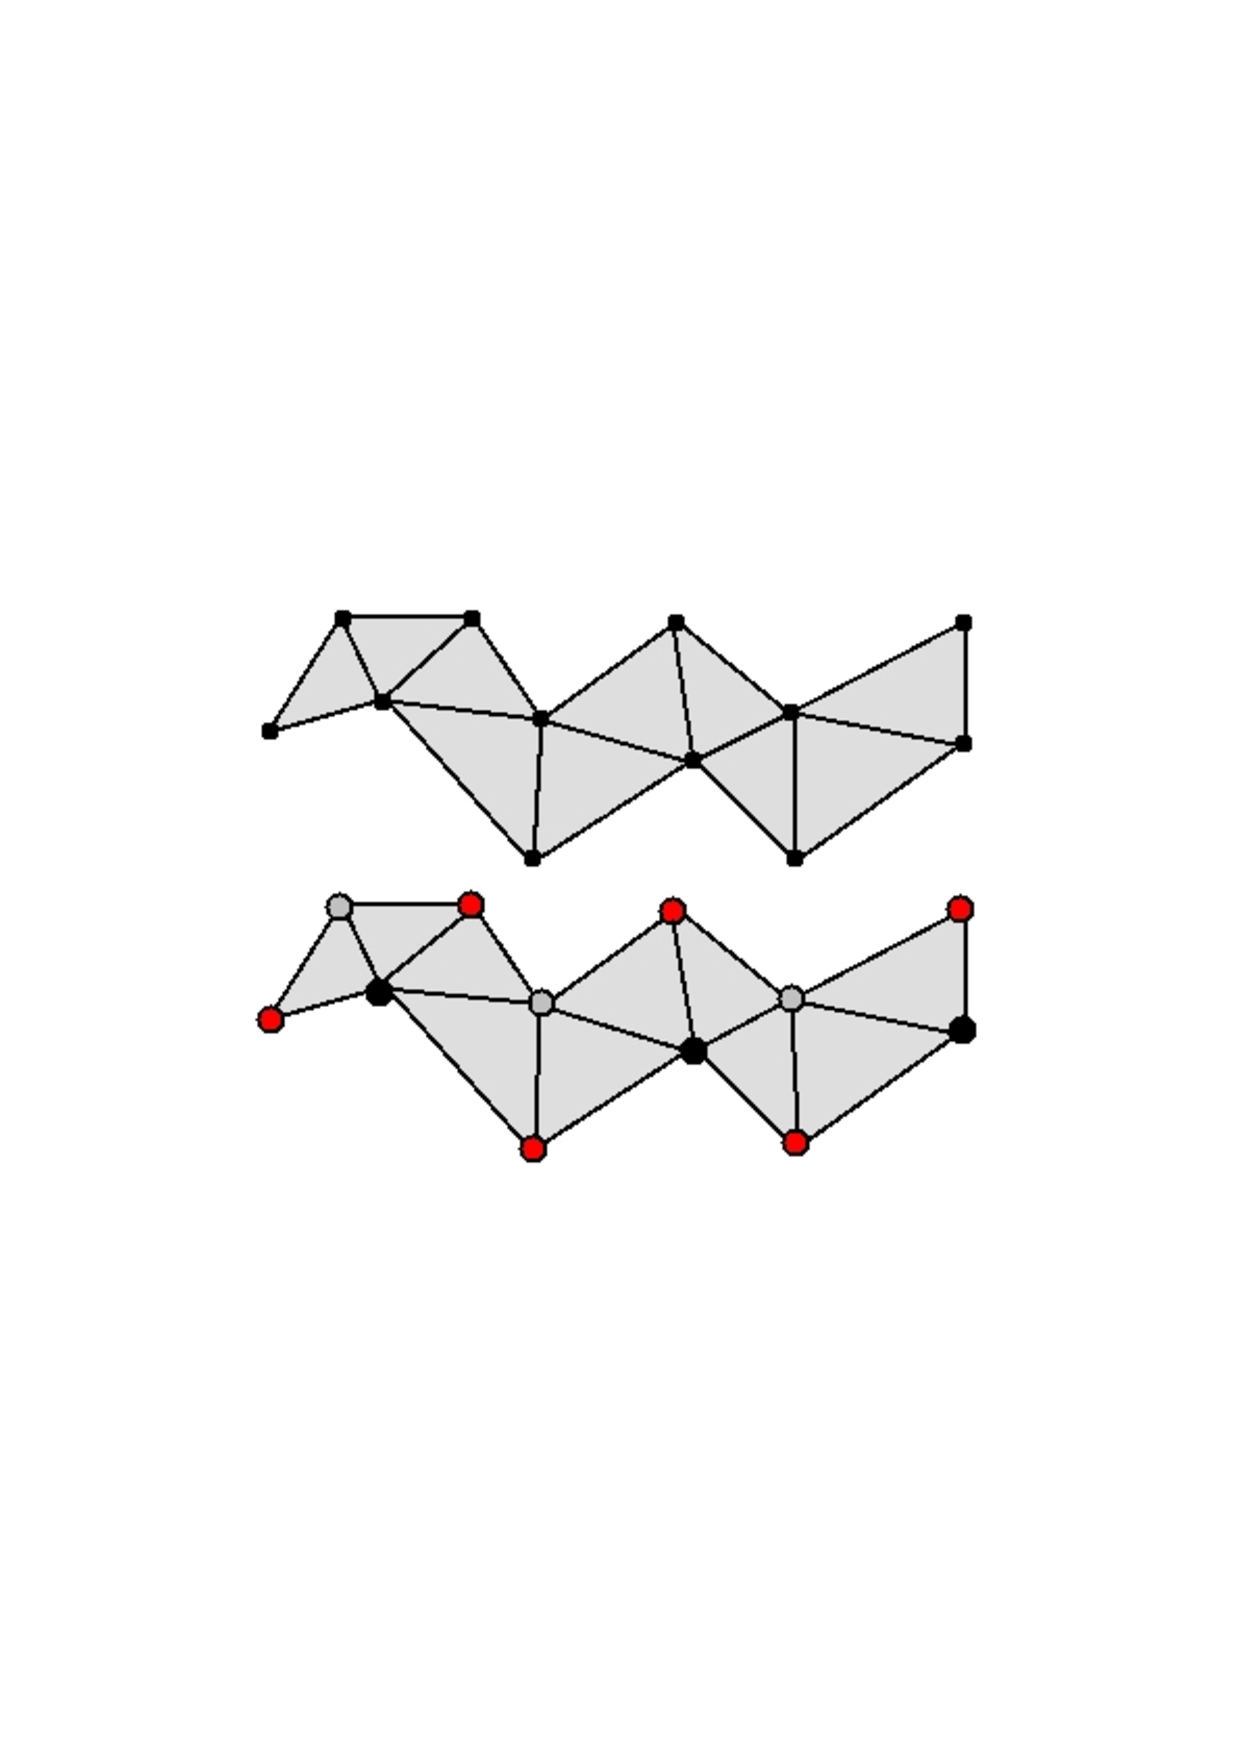
\includegraphics[width=0.4\textwidth]{lectures/161118/pix/Vertexfaerbung}